The literature review is advancing at a very good pace. Our objective this year 
is to generate a video-to-spike train encoder. For this, the first approach was 
to use a biologically plausible functional model \cite{basab-model} that 
results in images being transformed into rank-ordered spikes 
\cite{thorpe-spike-rapid-processing}.

\begin{figure}[hbt]
  \centering
  \begin{subfigure}[b]{0.15\textwidth}
    \centering
    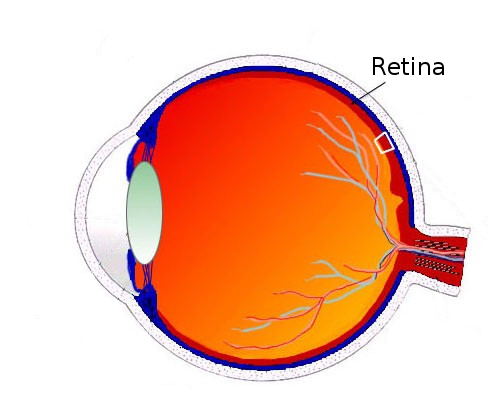
\includegraphics[width=\textwidth,valign=t]{Sagschem}
    \caption{Eye schematics}
    \label{sub-fig-eye-schematics}
  \end{subfigure}
  \begin{subfigure}[b]{0.15\textwidth}
    \centering
    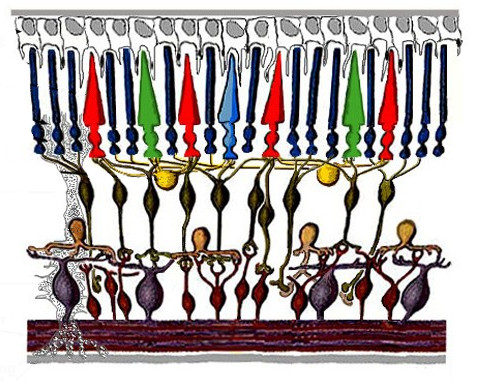
\includegraphics[angle=270,width=\textwidth,valign=t]{schem}
    \caption{Retina}
    \label{sub-fig-retinal-layers}
  \end{subfigure}
  \begin{subfigure}[b]{0.15\textwidth}
    \centering
    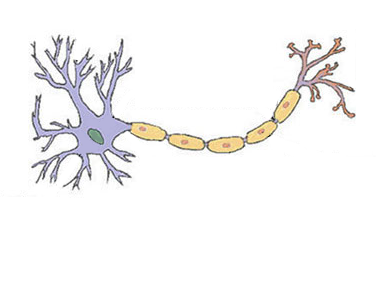
\includegraphics[width=\textwidth,valign=t]{Neuron-___-wikimedia-org}
    \caption{Neuron}
    \label{sub-fig-neuron}
  \end{subfigure}
  
  \caption{Anatomy of the (human) eye }
  \label{fig-basic-eye-anatomy}
\end{figure}

The retina is a thin layer of neural cells located in the eye (Fig. 
\ref{fig-basic-eye-anatomy}), it is responsible
for the sensing, processing and transmitting visual input\cite{webvision}. 
At its deepest layer, the retina has a millions of cells known as 
photoreceptors (right of Fig. \ref{sub-fig-retinal-layers}), they are in charge 
of transforming light into electrical 
signals. After this step there are three layers of neurons that 
perform different computations such as lateral inhibition or on/off 
centre-off/on surround behaviour (left of Fig. \ref{sub-fig-retinal-layers})
\cite{webvision, basab-model}. A small area 
at the centre of the retina has very few obstacles to obtain light and has high
resolution, this area is known as the \emph{foveal pit} (small depression on 
the right of Fig. \ref{sub-fig-eye-schematics}).

\begin{figure}[hbt]
  \centering
  \begin{subfigure}[t]{0.15\textwidth}
    \centering
    \captionsetup{justification=centering,margin=0.1cm}
    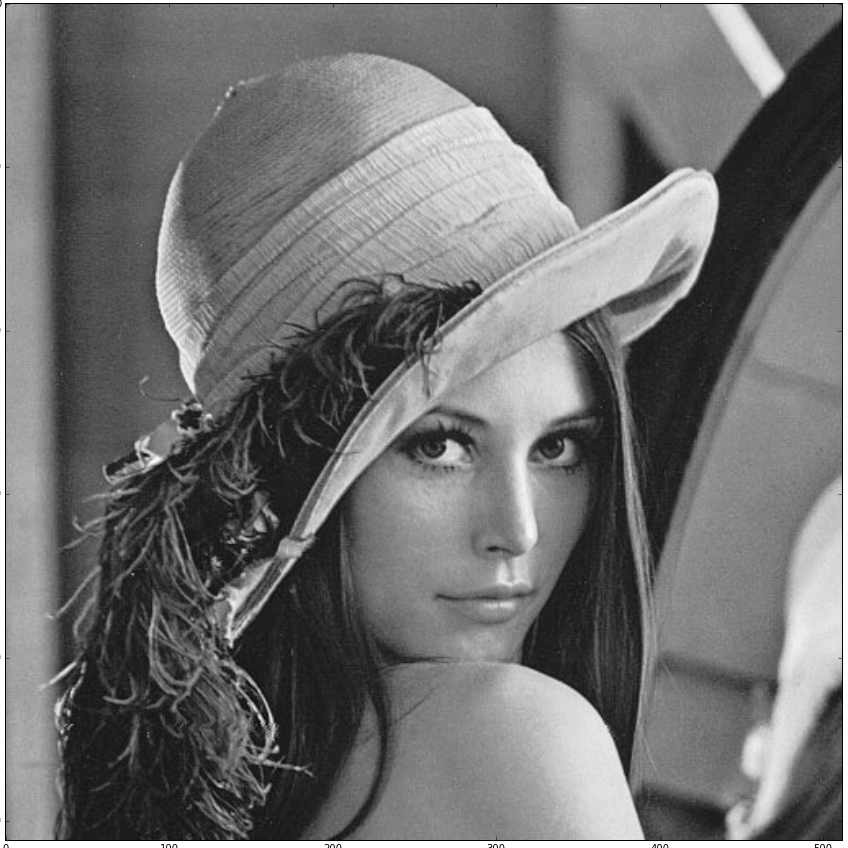
\includegraphics[width=\textwidth]{./Lena-gray}
    \caption{Original image}
    \label{pic-lena}
  \end{subfigure}
  \begin{subfigure}[t]{0.15\textwidth}
    \centering
    \captionsetup{justification=centering,margin=0.1cm}
    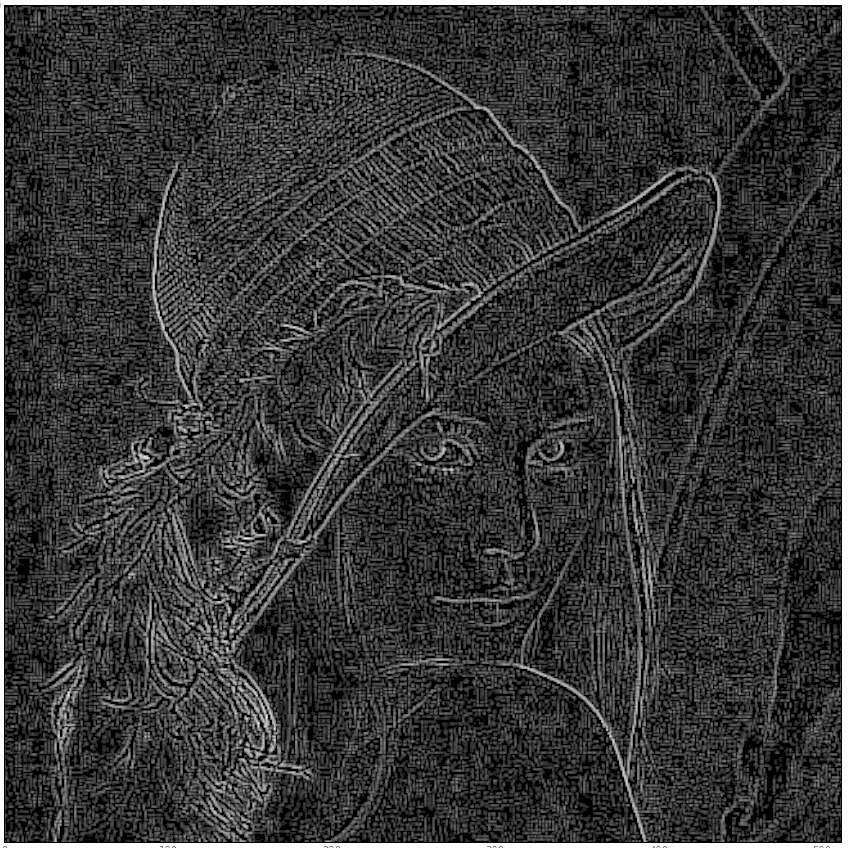
\includegraphics[width=\textwidth]{./Lena-midget_off}
    \caption{Midget OFF-centre}
    \label{pic-lena-M-OFF}
  \end{subfigure}
  \begin{subfigure}[t]{0.15\textwidth}
    \centering
    \captionsetup{justification=centering,margin=0.1cm}
    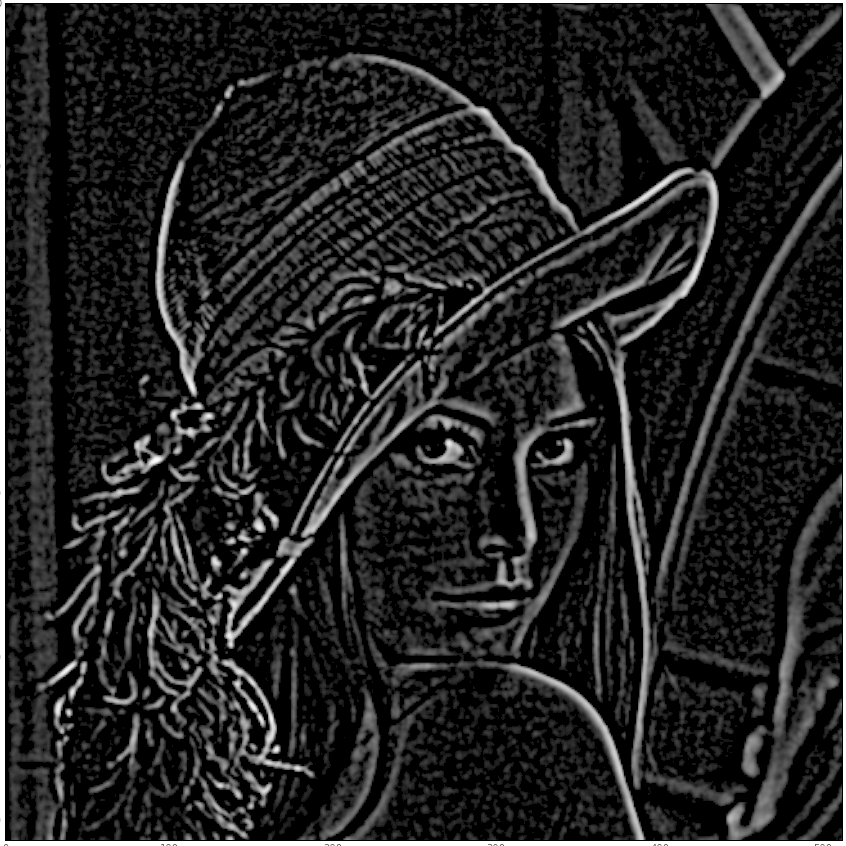
\includegraphics[width=\textwidth]{./Lena-midget_on}
    \caption{Midget ON-centre}
    \label{pic-lena-M-ON}
  \end{subfigure}
  \begin{subfigure}[t]{0.15\textwidth}
    \centering
    \captionsetup{justification=centering,margin=0.1cm}
    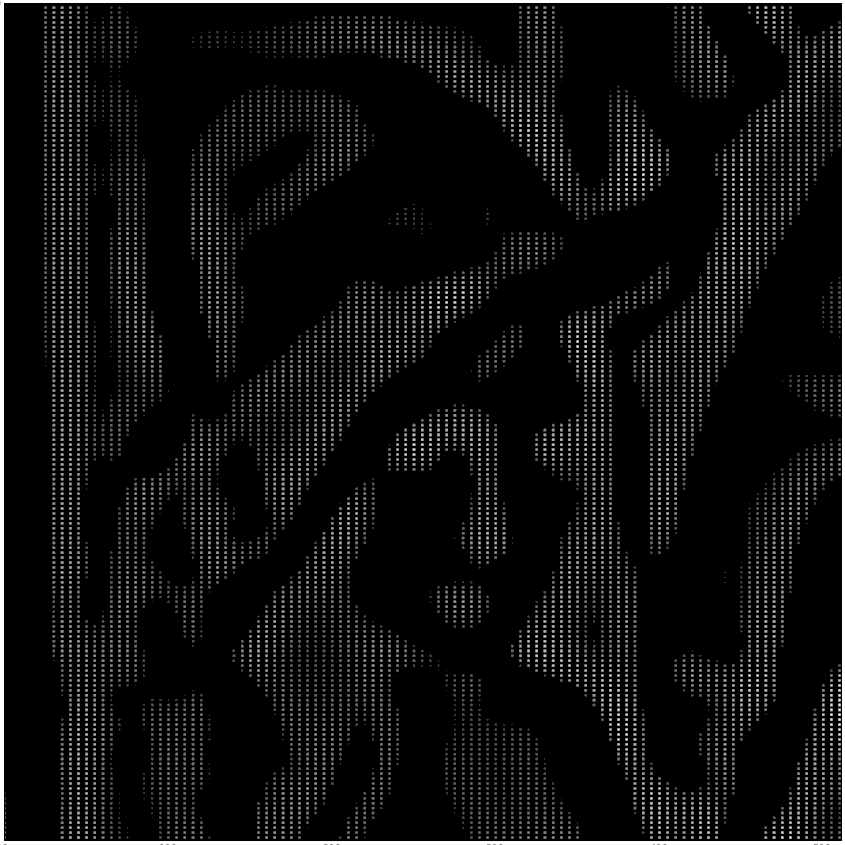
\includegraphics[width=\textwidth]{./Lena-parasol_off}
    \caption{Parasol OFF-centre}
    \label{pic-lena-P-OFF}
  \end{subfigure}
  \begin{subfigure}[t]{0.15\textwidth}
    \centering
    \captionsetup{justification=centering,margin=0.1cm}
    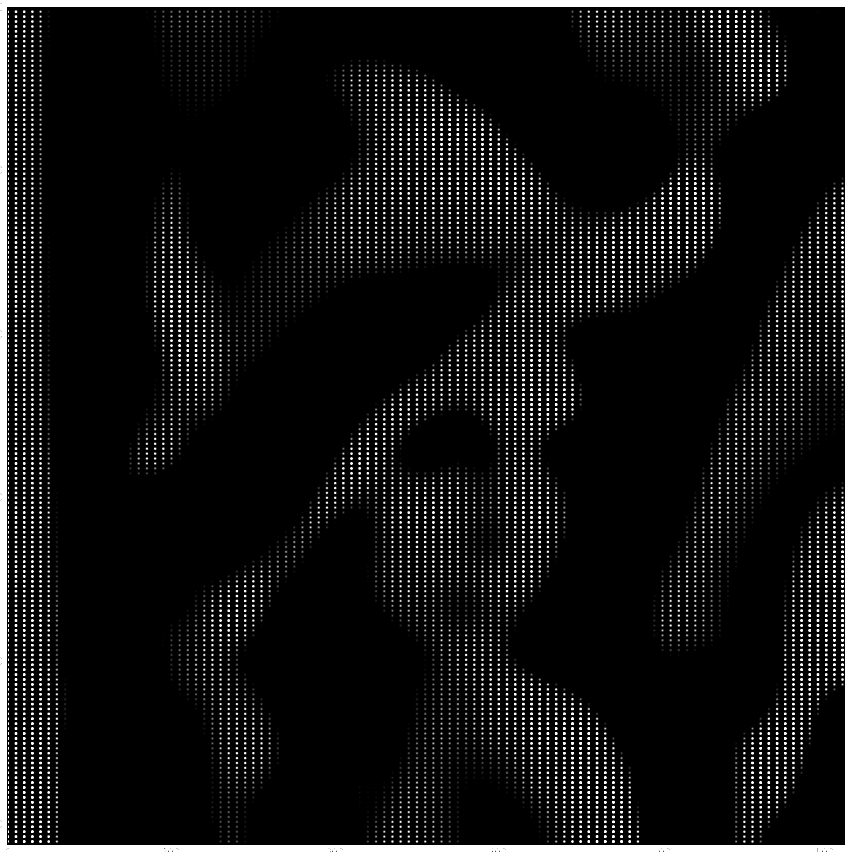
\includegraphics[width=\textwidth]{./Lena-parasol_on}
    \caption{Parasol ON-centre}
    \label{pic-lena-P-ON}
  \end{subfigure}
  \caption{Results of simulating ganglion cells (convoluted images are enhanced for better contrast)}
  \label{fig-convolution-results}
\end{figure}
This algorithm models the foveal pit, first we perform a two-dimensional 
discrete \emph{convolution} of the current frame with four \emph{kernels} 
(Table \ref{tab-kernel-specs}) which represent four types of ganglion cells; 
each cell type is modelled using a Difference of Gaussian (DoG, Eq. 
\ref{eq-dog}).
\begin{equation}
\label{eq-dog}
DoG_w(x,y) = \pm\frac{1}{2\pi\sigma_{w,c}^2}e^{\frac{-(x^2 + y^2)}{2\sigma_{w,c}^2}}
\mp\frac{1}{2\pi\sigma_{w,s}^2}e^{\frac{-(x^2 + y^2)}{2\sigma_{w,s}^2}}
\end{equation}
where $\sigma_{w,c}$ and $\sigma_{w,s}$ are the standard deviation for the 
centre and surround components of the DoG at scale $w$ (cell type). The signs 
will be ($-$,$+$) if the ganglion cell is OFF-centre and ($+$,$-$) if it is 
ON-centre.\\
Every pixel in the convoluted images (Fig. \ref{fig-convolution-results}) 
represent a spike emission time, the higher the pixel value, the sooner the 
spike will be sent out.
\begin{table}[htb]
  \caption{Simulation parameters for ganglion cells}
  \centering
%  \begin{TAB}(r,1em,1.5em){|c|c|c|c|c|}{|c|c|c|c|c|} 
  \begin{tabular}{l c c c c}
    \begin{minipage}{1.2cm}Cell type \end{minipage}& 
    \begin{minipage}{1cm} \centering Matrix width \end{minipage}&  
    \begin{minipage}{1.3cm}\centering Centre std. dev. ($\sigma_c$)\end{minipage} & 
    \begin{minipage}{1.3cm}\centering Surround std. dev. ($\sigma_s$)\end{minipage} & 
    \begin{minipage}{1.2cm}\centering Sampling resolution\end{minipage} \\
    \hline
    \begin{minipage}{1.2cm}\vspace*{0.1cm} Midget Off-centre \vspace*{0.005cm} \end{minipage}& 
    \begin{minipage}{1cm}\centering$3$ \end{minipage}& 
    $0.8$ & $6.7 \times \sigma_c$ &  
    \begin{minipage}{1.4cm}columns: 1, rows: 1\end{minipage}\\
    \begin{minipage}{1.2cm} Midget On-centre \vspace*{0.005cm}\end{minipage} & 
    \begin{minipage}{1cm}\centering $11$ \end{minipage}& 
    $1.04$ & $6.7 \times \sigma_c$ &  
    \begin{minipage}{1.4cm}columns: 1, rows: 1\end{minipage}\\
    \begin{minipage}{1.2cm}Parasol Off-centre \vspace*{0.005cm}\end{minipage} & 
    \begin{minipage}{1cm}\centering $61$ \end{minipage}& 
    $8$ & $4.8 \times \sigma_c$ & 
    \begin{minipage}{1.4cm} columns: 5, rows: 3 \end{minipage}\\
    \begin{minipage}{1.2cm} Parasol On-centre \vspace*{0.005cm}\end{minipage} & 
    \begin{minipage}{1cm}\centering $243$\end{minipage} &
    $10.4$ & $4.8 \times \sigma_c$ & 
    \begin{minipage}{1.4cm} columns: 5, rows: 3 \end{minipage}
%  \end{TAB} 
  \end{tabular}
  \label{tab-kernel-specs}
\end{table}
Different ways of performing convolutions on a GPU where implemented, the naïve
does a discrete convolution with the full kernels; for the biggest kernel 
($243\times243$ elements) we were unable to fit it into one of the fast memory
locations of the GPU. We decompose the DoG into two horizontal and two vertical
convolution kernels to perform a separated convolution. This method works best 
on kernels bigger than $3\times3$. Last approach, \emph{Tiled Convolution} is 
reported by Advanced Micro Devices (AMD) in \cite{tiled-convolution}. They only 
do kernels of size $3\times3$, but we have an $11\times11$ convolution working; 
we are still developing solutions for the larger kernels.
Convolution alone is a compute intensive task and we 
obtain about 12 frames-per-second (FPS) on videos with $640\times360$ 8-bit 
grayscale pixel resolution. Encoding was carried out using a desktop computer 
running 64-bit GNU/Linux, with a Core i5-4570 4-core CPU @ 3.20GHz processor 
with 8 GBytes of 64-bit DDR3 RAM @ 1600MHz and a GeForce GT 720 GPU with 192 
CUDA cores @ 797 MHz, 1 GBytes of 64-bit DDR3 RAM @ 1800 MHz. %\\

\begin{table}
  \begin{center}
      \caption{Performance comparison.}
      \bgroup
      \def\arraystretch{1.2}
      \begin{tabular}{l c c c c}
  %      \begin{minipage}{1.2cm} \vspace*{0.2cm}Algorithm \vspace*{0.001cm}\end{minipage}& 
        &
        \begin{minipage}{1.2cm}Midget Off-centre\vspace*{0.05cm}\end{minipage} & 
        \begin{minipage}{1.2cm}Midget On-centre\vspace*{0.05cm}\end{minipage}& 
        \begin{minipage}{1.2cm}Parasol Off-centre\vspace*{0.05cm}\end{minipage}& 
        \begin{minipage}{1.2cm}Parasol On-centre\vspace*{0.05cm}\end{minipage}\\
        \hline 
        \vspace*{0.1cm}
        Naïve     & 0.0009s & 0.0031s & 0.0587s & N/A$^1$ \\ 
        Separated & 0.0029s & 0.0055s & 0.0172s & 0.0472s \\ 
        Tiled     & 0.0019s & 0.0027s & N/A$^2$ & N/A$^2$\\
      \end{tabular} 
      \egroup

  {
    \footnotesize $^1$ Unable to fit convolution kernel into constant memory.\\
                  $^2$ Coding optimizations are still in progress.
  }
  \end{center}
\end{table}
  %\vspace*{-pt}


In the retina, redundancy of information is reduced via lateral inhibition 
prior to any ganglion cell activity. In this algorithm, we perform a correction 
is on the convolved images by adjusting the convoluted image's weights 
according to the correlation between convolution kernels. The results of using
correction (Fig. \ref{pic-unfiltered-spikes}) or not (Fig. 
\ref{pic-100pc-spikes}) show that the convolution stage can only provide 
redundant information. Furthermore using only 30\% of the corrected weights, 
enough visual information is transmitted to reconstruct the
original image \cite{basab-model}.

\begin{figure}
  \centering
  \begin{subfigure}[t]{0.15\textwidth}
    \centering
    \captionsetup{justification=centering,margin=0.1cm}
    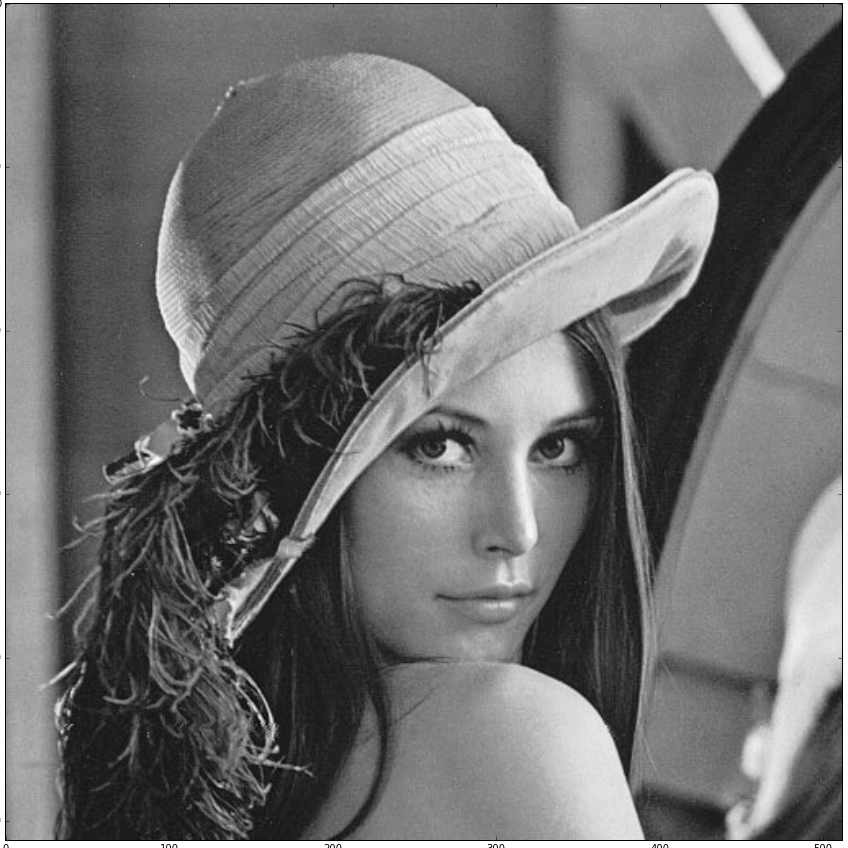
\includegraphics[width=\textwidth]{./Lena-gray}
    \caption{Original image}
    \label{pic-original-lena}
  \end{subfigure}
  \begin{subfigure}[t]{0.15\textwidth}
    \centering
    \captionsetup{justification=centering,margin=0.1cm}
    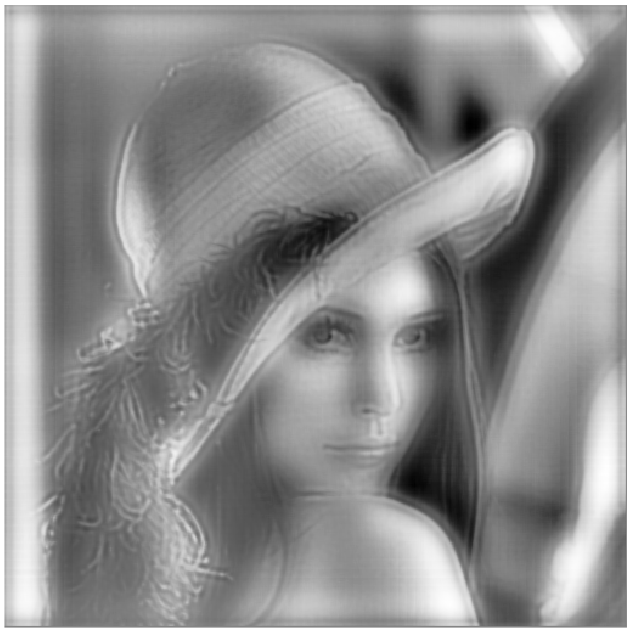
\includegraphics[width=\textwidth]{./final_results-unfiltered}
    \caption{100\% of \\raw spikes}
    \label{pic-unfiltered-spikes}
  \end{subfigure}
  %        \hfill
  \begin{subfigure}[t]{0.15\textwidth}
    \centering
    \captionsetup{justification=centering,margin=0.1cm}
    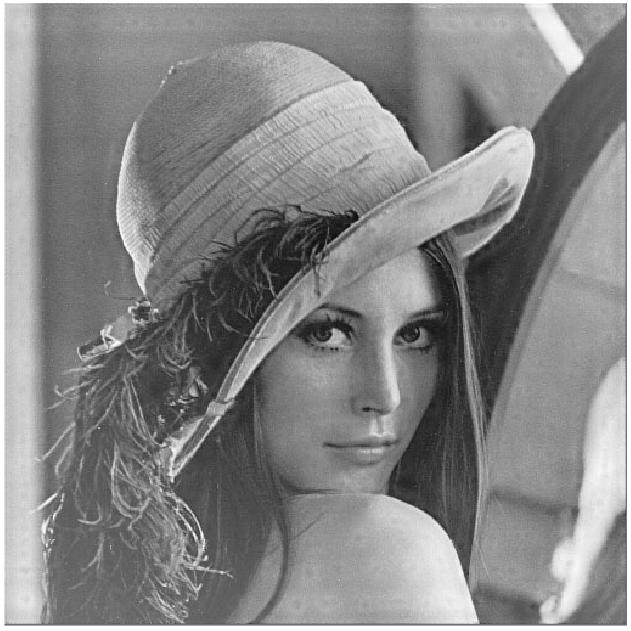
\includegraphics[width=\textwidth]{./final_results-focal-100}
    \caption{100\% of \emph{corrected} spikes}
    \label{pic-100pc-spikes}
  \end{subfigure}
%  \begin{subfigure}[t]{0.15\textwidth}
%    \centering
%    \captionsetup{justification=centering,margin=0.1cm}
%    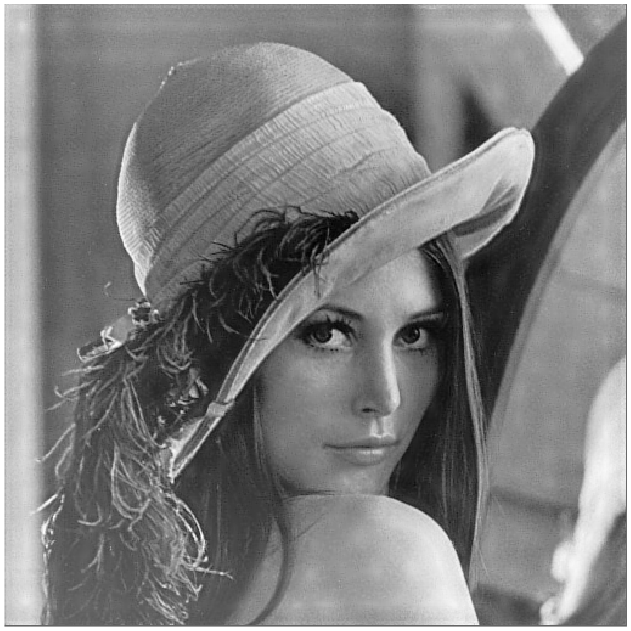
\includegraphics[width=\textwidth]{./final_results-focal-30pc}
%    \caption{\\30\% of \emph{corrected} spikes}
%    \label{pic-30pc-spikes}
%  \end{subfigure}
  \caption{Results of reconstruction procedure}
  \label{fig-reconstruction}
\end{figure}
Correcting the spikes for redundancy is a highly time consuming task which
might be better suited for event-based programming, such as the one found on 
the SpiNNaker platform. We are still working on an implementation for this 
approach.

A second way of encoding is to simulate the early stages of the retina, which
sense changes in intensity on the photoreceptors. This is quite similar to what 
real Dynamic Vison Sensors (DVS, \cite{aer-retina-bernabe,dvs-zurich}) do but 
with limited dynamic range and lower temporal resolution. The main advantage is 
that no specialized hardware is needed and the operation is so fast that any 
recent computer should be able to do it. For this type of encoding procedure we 
hypothesize that the bigger the change, the sooner a cell would spike and, 
thus, we can obtain a spike timings given the difference of two video frames. 
So far we can process about 20 and 25 FPS using a Numpy and an OpenCL backend, 
respectively (using the same hardware set-up previously described). Although 
it's currently a good approximation, more research on this algorithm is needed 
to better approximate to biology. 


